% ==============================================================================
% FYDP-I Roll-Up / Pull-Up Banner
% "Solving the Lorenz ODE System Using Optimal ANN Architectures"
% United International University - Department of CSE
%
% PRINT SIZE: 800 x 2000 mm (most common roll-up size).
%   For other standards change \geometry below:
%     850 x 2000 -> paperwidth=85cm   |  1000 x 2000 -> paperwidth=100cm
%     1200 x 2000 -> paperwidth=120cm
%
% ROLL-UP SAFE ZONE: the lowest ~120-150 mm of a pull-up banner curls into the
%   base cassette and the top ~50 mm sits under the rail. Critical content
%   (title, question, key result) is kept in the upper/middle bands; the footer
%   band at the bottom is intentionally low-priority (references + QR).
%
% Teal theme matched to the institutional reference poster.
% Compile: pdflatex banner.tex
% ==============================================================================
\documentclass[
  25pt,
  a0paper,            % overridden below by \geometry
  portrait,
  margin=22mm,
  innermargin=16mm,
  blockverticalspace=15mm,
  colspace=14mm,
  subcolspace=12mm
]{tikzposter}

% ---- custom roll-up banner page size (overrides a0paper) ----
\geometry{paperwidth=80cm, paperheight=200cm}

\usepackage{graphicx}
\usepackage{amsmath,amssymb}
\usepackage{qrcode}
\graphicspath{{./figures/}}

% ---------------------------------------------------------------- colours
\definecolor{tealDark}{RGB}{62,124,116}
\definecolor{tealMid}{RGB}{143,196,189}
\definecolor{tealSoft}{RGB}{206,231,228}
\definecolor{ink}{RGB}{32,46,44}
\definecolor{accent}{RGB}{223,150,64}

\usetheme{Default}

\definecolorstyle{LorenzTeal}{
  \definecolor{colorOne}{RGB}{62,124,116}
  \definecolor{colorTwo}{RGB}{143,196,189}
  \definecolor{colorThree}{RGB}{206,231,228}
}{
  \colorlet{backgroundcolor}{white}
  \colorlet{framecolor}{colorOne}
  \colorlet{titlefgcolor}{white}
  \colorlet{titlebgcolor}{colorOne}
  \colorlet{blocktitlebgcolor}{colorTwo}
  \colorlet{blocktitlefgcolor}{ink}
  \colorlet{blockbodybgcolor}{white}
  \colorlet{blockbodyfgcolor}{ink}
  \colorlet{innerblocktitlebgcolor}{colorThree}
  \colorlet{innerblocktitlefgcolor}{ink}
  \colorlet{notebgcolor}{colorThree}
  \colorlet{notefrcolor}{colorOne}
}
\usecolorstyle{LorenzTeal}

\usebackgroundstyle{Empty}
\usetitlestyle{Filled}
\useblockstyle{Default}
\tikzposterlatexaffectionproofoff   % remove the "LaTeX TikZposter" watermark

% ---------------------------------------------------------------- title matter
\title{\parbox{\linewidth}{\centering Solving the Lorenz ODE System\\[4pt]
  Using Optimal ANN Architectures}}
\author{\mbox{Ikramul Hasan Moral} \textbullet\ \mbox{Md.\ Abu Bakar} \textbullet\
  \mbox{Samiur Rahman Omlan} \textbullet\ \mbox{Fariha Islam} \textbullet\ \mbox{Md.\ Touhidul Islam}}
\institute{Department of Computer Science and Engineering, United International University \\[3pt]
  \textbf{Supervisor:} Dr.\ Muhammad Nomani Kabir, Professor, Dept.\ of CSE \quad \textbullet \quad \textbf{Course Teacher:} Dr.\ Md.\ Motaharul Islam, Professor, Dept.\ of CSE}
\titlegraphic{
\includegraphics[width=6.5cm]{uiu.png}}

\begin{document}
\maketitle[width=0.96\linewidth]

\begin{columns}
\column{1}   % single full-width column -> vertical banner narrative

% ---------------------------------------------------------------- 1. INTRO
\block{Introduction \& Central Question}{
  Coupled nonlinear ODEs such as the \textbf{Lorenz-1960} system --- an early
  three-equation meteorological model --- rarely admit closed-form solutions.
  Classical Runge--Kutta solvers are accurate but \textbf{mesh-dependent} and
  re-integrate step-by-step for every query. A trained network can instead learn
  the continuous map $t\mapsto(x,y,z)$ in one shot, yet most neural-ODE work leans
  on physics-informed losses or operator learning.
  \vspace{3mm}

  \innerblock{Central question}{
    Can a \textbf{plain feedforward ANN} --- trained only on numerical data, with
    \emph{no physics in the loss} --- approximate the Lorenz-1960 solution, and
    \emph{which architecture does it best}?
  }
  \vspace{3mm}

  \textbf{Objectives.}\enspace
  (i)~build a trusted RK4\,$+$\,SciPy reference and cross-validate it;\quad
  (ii)~vary \textbf{depth $\times$ width $\times$ activation} systematically;\quad
  (iii)~score accuracy vs.\ cost (MSE, MAE, max error, train/infer time);\quad
  (iv)~benchmark the best plain ANN against PINN / DeepONet results.
}

% ---------------------------------------------------------------- 2. BACKGROUND
\block{Background: System \& Network}{
  \begin{minipage}[c]{0.47\linewidth}
    Three coupled nonlinear ODEs; with $k=2,\ l=1$:
    \[
    \begin{aligned}
      \dot{x}&=kl\!\left(\tfrac{1}{k^2+l^2}-\tfrac{1}{k^2}\right)yz\\[3pt]
      \dot{y}&=kl\!\left(\tfrac{1}{l^2}-\tfrac{1}{k^2+l^2}\right)xz\\[3pt]
      \dot{z}&=\tfrac{kl^2}{2}\!\left(\tfrac{1}{k^2}-\tfrac{1}{l^2}\right)xy
    \end{aligned}
    \]
    \vspace{1mm}

    Reduced form: $\dot{x}=-0.1\,yz,\ \dot{y}=1.6\,xz,\ \dot{z}=-0.75\,xy$.\\[3pt]
    {\small Initial state $x_0{=}0.5,\ y_0{=}0.75,\ z_0{=}1$, on $t\in[0,1]$.}
  \end{minipage}\hfill
  \begin{minipage}[c]{0.50\linewidth}
    \centering
    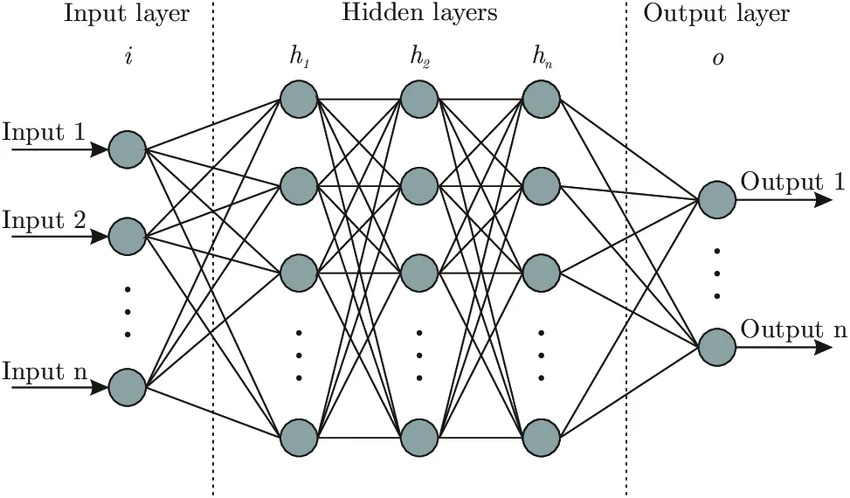
\includegraphics[width=\linewidth]{ann_architecture.jpg}\\[3pt]
    {\small Plain feedforward ANN: learns $t\mapsto(x,y,z)$ by backpropagation.
      PINNs appear only as a literature benchmark, not as part of this model.}
  \end{minipage}
}

% ---------------------------------------------------------------- 3. METHODOLOGY
\block{Methodology --- Two-Phase Study (69 Controlled Runs)}{
  \begin{minipage}[t]{0.49\linewidth}
    \innerblock{Phase 1 --- Architecture search}{
      depth $\{1,2,3,4\}\ \times$ width $\{20,50,100\}\ \times$
      activation $\{$tanh, ReLU, sigmoid, GELU, Swish$\}$\\[3pt]
      \centering\textbf{= 60 runs} \;(Adam held fixed)
    }
  \end{minipage}\hfill
  \begin{minipage}[t]{0.49\linewidth}
    \innerblock{Phase 2 --- Optimizers}{
      3 best Phase-1 architectures $\times$
      \{Adam, L-BFGS, SGD\,$+$\,momentum\}\\[3pt]
      \centering\textbf{= 9 runs}
    }
  \end{minipage}

  \vspace{3mm}
  \centering
  \textbf{69 controlled experiments} --- the split cleanly separates
  \emph{architecture} effects from \emph{optimizer} effects.
  \vspace{4mm}

  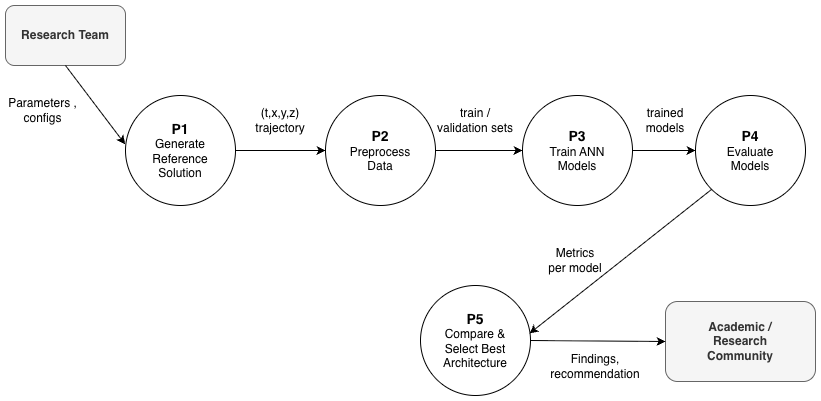
\includegraphics[width=1.0\linewidth]{dfd_level1.png}\\[2pt]
  {\small Data pipeline: generate $\to$ preprocess $\to$ train $\to$ evaluate $\to$ select.}
}

% ---------------------------------------------------------------- 4. RESULT
\block{Numerical Baseline \& Validation}{
  The reference trajectory is produced by two independent solvers and cross-checked
  \emph{before any ANN sees it}: a custom \textbf{RK4} integrator
  ($h{=}10^{-3}$, 1001 points) and \textbf{SciPy DOP853} ($\mathrm{rtol}{=}10^{-10}$),
  split 80/20 for train/validation (seed 42).
  \vspace{3mm}

  \centering
  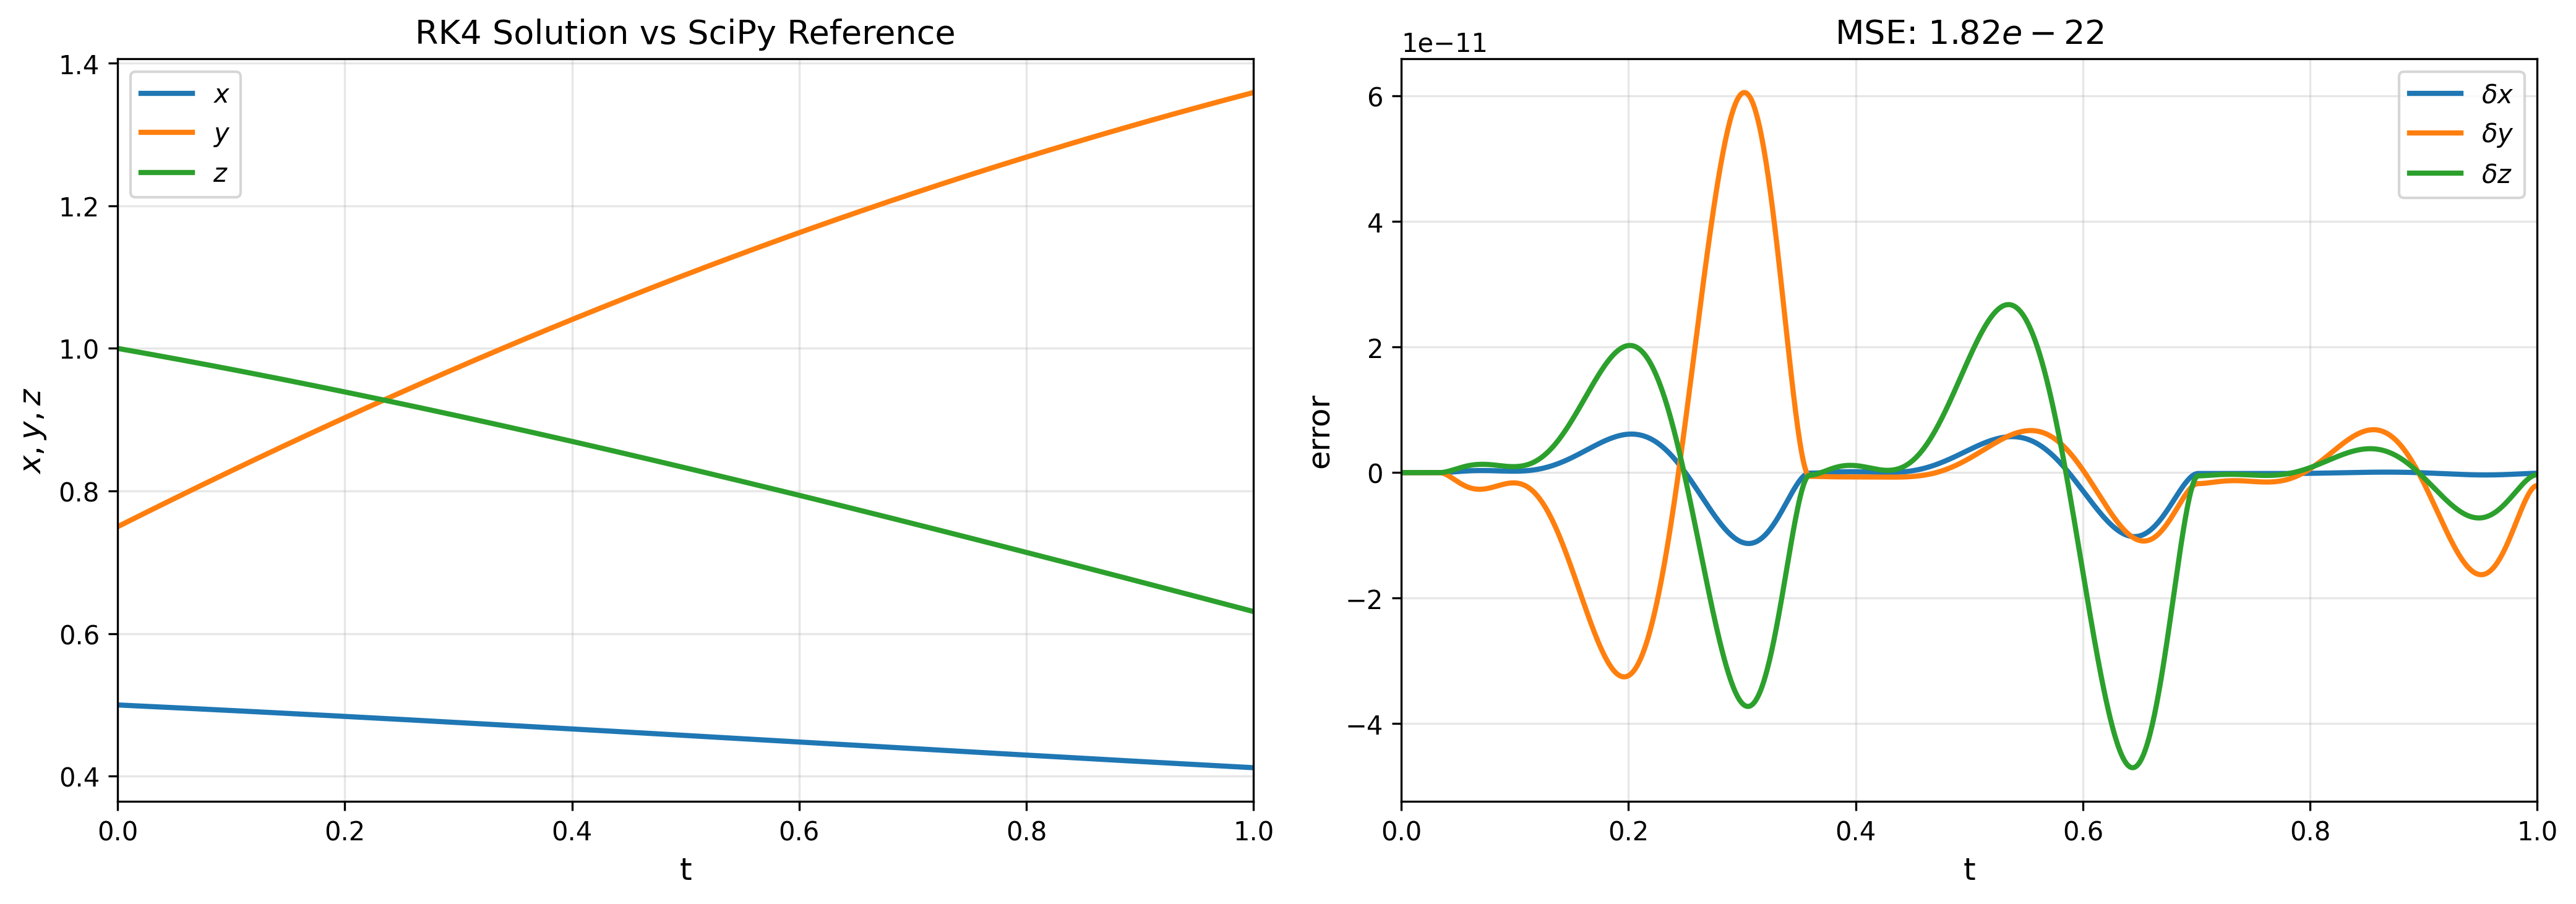
\includegraphics[width=1.0\linewidth]{lorenz1960_comparison.png}\\[3pt]
  \raggedright
  The two solvers agree to \textbf{MSE $\approx 1.8\times10^{-22}$}, far below the
  $10^{-10}$ target --- a defensible \textbf{ground truth} for all FYDP-II ANN training.
}

% ---------------------------------------------------------------- 5. STATUS
\block{Status (FYDP-I) \& Future Work}{
  \textbf{Delivered this stage:} research question framed; 17-paper review with an
  explicit gap; two-phase design (69 runs) locked; dual-solver baseline verified.
  \textbf{No accuracy claims are made} until FYDP-II experiments produce evidence.
  \begin{itemize}
    \item Build the ANN training pipeline; run Phase 1 (60), then Phase 2 (9).
    \item Repeat seeds for stability; test denser grids and new initial conditions.
    \item Compare directly with PINN / operator-learning baselines.
  \end{itemize}
}

% ---------------------------------------------------------------- 6. FOOTER
\block{Key References \& Contact}{
  \begin{minipage}[c]{0.72\linewidth}
    \small
    [1]~Lorenz (1960), \textit{Tellus} 12(3).\quad
    [2]~Matthews \& Bihlo (2024), PinnDE.\quad
    [3]~Raissi et al.\ (2019), \textit{J.\ Comput.\ Phys.}\ 378.\par
    [4]~Lagaris et al.\ (1998), \textit{IEEE TNN} 9(5).\quad
    [5]~Lau \& Werth (2020), ODEN.\par
    \vspace{2mm}
    \normalsize \textbf{Team\_ParaDox} \quad \textbullet \quad Project repository \textbullet\ \texttt{github.com/ihmorol/fydp\_workspace}
  \end{minipage}\hfill
  \begin{minipage}[c]{0.24\linewidth}
    \centering
    \qrcode[height=3.2cm]{https://github.com/ihmorol/fydp_workspace}\\[2pt]
    {\small Scan for code \& data}
  \end{minipage}
}

\end{columns}

\end{document}
